\documentclass[12pt,titlepage,headings,oneside,openany]{book}
\usepackage{kotex}
\usepackage{graphicx}
\usepackage{epsfig}
\usepackage{epstopdf}
\usepackage{subfigure}
\usepackage{rotating}
\usepackage{enumitem}
\usepackage{amsfonts,amssymb}
\usepackage{pifont}
\usepackage{indentfirst}
\usepackage{lscape}
\usepackage{booktabs,longtable,adjustbox,caption,array}
\usepackage{soul}
\soulregister{\ref}{1}
\soulregister{\cite}{1}
\usepackage{xcolor}
\usepackage{fvextra}
\usepackage{algorithmic}
\usepackage{stfloats}
\usepackage{verbatim}
\usepackage[cmex10]{amsmath}
\usepackage{newlfont}
\usepackage{XThesis_skku_eng}
\usepackage[active]{srcltx}
\usepackage{notebook}
\usepackage{fancyhdr}
\usepackage{cite}
\usepackage[hyphens]{url}
\usepackage{array,tabularx}
\usepackage{bm,upgreek}
\usepackage{textcomp}
\usepackage{makecell,multirow}
\usepackage{ifpdf}
\usepackage{float}
\usepackage{placeins}
\usepackage{mathtools}
\usepackage{microtype}
\ifpdf
  \usepackage[CJKbookmarks]{hyperref}
  \hypersetup{hidelinks}
\else
  \usepackage[dvipdfm,CJKbookmarks]{hyperref}
  \hypersetup{hidelinks}
  \AtBeginDvi{\special{pdf: tounicode KSCms-UHC-UCS2}}
\fi
% Symmetric vertical margins for the thesis body.
% The previous template used a large positive \voffset and the default book-class
% chapter spacing, which pushed chapter titles far below the top of the page.
\usepackage[
  a4paper,
  top=25mm,
  bottom=25mm,
  left=36mm,
  right=36mm,
  includefoot,
  footskip=10mm
]{geometry}

% Place chapter headings at the top of the text area instead of adding the
% default 50 pt blank space used by the book class.
\makeatletter
\def\@makechapterhead#1{%
  \vspace*{0pt}%
  {\parindent \z@ \raggedright \normalfont
    \ifnum \c@secnumdepth >\m@ne
      \if@mainmatter
        \huge\bfseries \@chapapp\space \thechapter
        \par\nobreak
        \vskip 14\p@
      \fi
    \fi
    \interlinepenalty\@M
    \Huge \bfseries #1\par\nobreak
    \vskip 28\p@
  }}
\def\@makeschapterhead#1{%
  \vspace*{0pt}%
  {\parindent \z@ \raggedright \normalfont
    \interlinepenalty\@M
    \Huge \bfseries #1\par\nobreak
    \vskip 28\p@
  }}
\makeatother
\hfuzz2pt
\newlength{\defbaselineskip}
\setlength{\defbaselineskip}{\baselineskip}
\newcommand{\setlinespacing}[1]{\setlength{\baselineskip}{#1 \defbaselineskip}}
\newcommand{\doublespacing}{\setlength{\baselineskip}{2.0 \defbaselineskip}}
\newcommand{\singlespacing}{\setlength{\baselineskip}{\defbaselineskip}}
\newcommand{\todoexp}[1]{\textcolor{red}{[Planned/TBD: #1]}}
% TODO: Finalize thesis title after journal positioning and experiments.
\newcommand{\fairetitle}{FAIRE: Force-Aware Imitation with Residual-Removal-Aware Blending for CAD-Free Robotic Surface Repair}
\begin{document}
\setlinespacing{1.7}
\def\baselinestretch{1}
\pagestyle{fancy}
\fancyhf{}
\fancyfoot[C]{\thepage}
\renewcommand{\headrulewidth}{0pt}
\renewcommand{\footrulewidth}{0pt}
\pagenumbering{roman}
\tableofcontents
\clearpage
\phantomsection
\addcontentsline{toc}{chapter}{List of Tables}
\listoftables
\clearpage
\phantomsection
\addcontentsline{toc}{chapter}{List of Figures}
\listoffigures
\clearpage
\markboth{Abstract}{Abstract}
\chapter*{Abstract}
\addcontentsline{toc}{chapter}{Abstract}
\begin{center}
\Large\textbf{FAIRE: Force-Aware Imitation with Residual-Removal-Aware Blending for CAD-Free Robotic Surface Repair}
\end{center}

Localized surface defects must be removed selectively because unnecessary processing can damage intact material, whereas insufficient processing leaves the defect visible or functionally significant. Conventional perception-and-planning approaches can localize a defect and generate a geometric repair path, but defect geometry alone does not specify the process intensity, local repetition, desired contact behavior, or termination condition required for removal when depth, severity, and removal difficulty are not explicitly available. FAIRE therefore uses visual and force-conditioned imitation learning as an expert repair policy. From an image, robot state, and recent six-axis wrench history, the policy predicts short-horizon Cartesian pose and desired three-axis force trajectories that represent the operator's defect-dependent decisions about how to process, how much to process, where to repeat, and when to terminate. The desired contact force is a controller-level reference, and the demonstrated tangential feed velocity is preserved during this selective-removal stage.

Successful defect removal, however, does not guarantee a spatially uniform and smoothly restored surface. Concentrated processing can leave a local depression, nonuniform removal, turning-point overlap, or a visible boundary to the untreated surface. FAIRE therefore logs the actual executed pose, orientation, wrench, and velocity history and converts it into a Preston-model-based estimated material-removal map using a calibrated Preston coefficient and tool influence function. A target profile regularizes the defect-containing core toward a uniform target depth and smoothly decreases removal across an outer transition region. The difference between this profile and the estimated removal map defines the residual-removal demand.

A model-based planner generates a local CAD-free blending path and nominal process conditions from that demand. Admittance control compensates for unknown surface height, while bounded residual reinforcement learning adapts roll, pitch, and feed velocity during blending on unseen smooth curved surfaces. Velocity adaptation is residual-removal-aware and is not applied during expert imitation. Evaluation is planned through staged comparisons of expert imitation, force-history representations, removal-model calibration, blending, residual policies, and end-to-end repair. Quantitative findings will be populated only from completed experiments.

\vspace{0.5cm}
\noindent\textbf{Keywords:} Robotic Surface Repair, Force-Aware Imitation Learning, Material-Removal Estimation, Model-Based Blending, Admittance Control, Residual Reinforcement Learning, CAD-Free Surface Processing

\pagenumbering{arabic}
\setcounter{page}{1}
\markboth{Introduction}{Introduction}
\chapter{Introduction}
\section{Background and Motivation}
Robotic surface finishing, including polishing, sanding, grinding, and buffing, is a physically demanding and quality-sensitive manufacturing process. The final result depends not only on the nominal path of the robot but also on contact pressure, sliding velocity, dwell time, tool orientation, abrasive state, and local surface geometry. Conventional fixed-path automation can achieve high repeatability on structured parts, yet it is difficult to transfer to high-mix products containing large smooth regions, sharp boundaries, concave transitions, narrow features, and reflective hardware.

The dominant automation pipeline combines three-dimensional perception or CAD with explicit coverage planning and compliant control. A surface model provides normals, curvature, boundaries, and collision geometry; a planner generates a raster, iso-parametric, geodesic, or region-based trajectory; and a force, impedance, or admittance controller maintains contact. Recent work has improved uniform coverage, segmentation, contact-point switching, and manipulator feasibility~\cite{schneyer2023segmentation,tafuro2024autonomous,gong2025uniform,wang2025coverage,pusnik2025region}. These methods are effective on broad and continuously observable surfaces because product variation can be represented by a new CAD or mesh while reusing the same planning algorithm.

However, full-product polishing exposes two unresolved limitations. First, a path that covers a mathematical surface does not necessarily cover the surface with the physical tool. A polishing pad has a finite and deformable footprint. The path spacing must therefore depend on the effective tool width, overlap ratio, surface curvature, tool tilt, and boundary offset. The tool center point (TCP) is a point and has no width; throughout this thesis, the phrase \emph{tool width} refers to the effective contact footprint of the polishing tool. Second, geometric coverage does not guarantee uniform material removal because the actual pressure and sliding velocity vary during execution. According to the Preston relation, the local removal rate is approximately proportional to their product~\cite{preston1927theory}.

A third challenge occurs at edges, cutaways, narrow transitions, and hardware-adjacent regions. Modern geometric planners can introduce region-specific strategies and move the tool contact point, but their rule and parameter complexity grows with the number of local contact modes~\cite{schneyer2023segmentation}. In repair and reconditioning, the geometry is further combined with product-specific scratches, oxidation, loss of gloss, and wear. The desired approach direction, tool tilt, contact-force reduction, repeated short strokes, and termination time may be easier for a skilled operator to demonstrate than to specify through a universal analytical objective.

This thesis therefore proposes a hybrid architecture. Tool-footprint-aware full-coverage planning is used for the entire CAD surface and broad regular regions. Reinforcement learning optimizes the sliding velocity along the geometric path while the path and low-level admittance controller remain fixed. Force-aware imitation learning generates local pose--force trajectories for difficult segments. Finally, object-centric and predictive feature masking is introduced to reduce the influence of reflections, background clutter, and irrelevant image regions on the imitation-learning policy.

\begin{figure}[t]
    \centering
    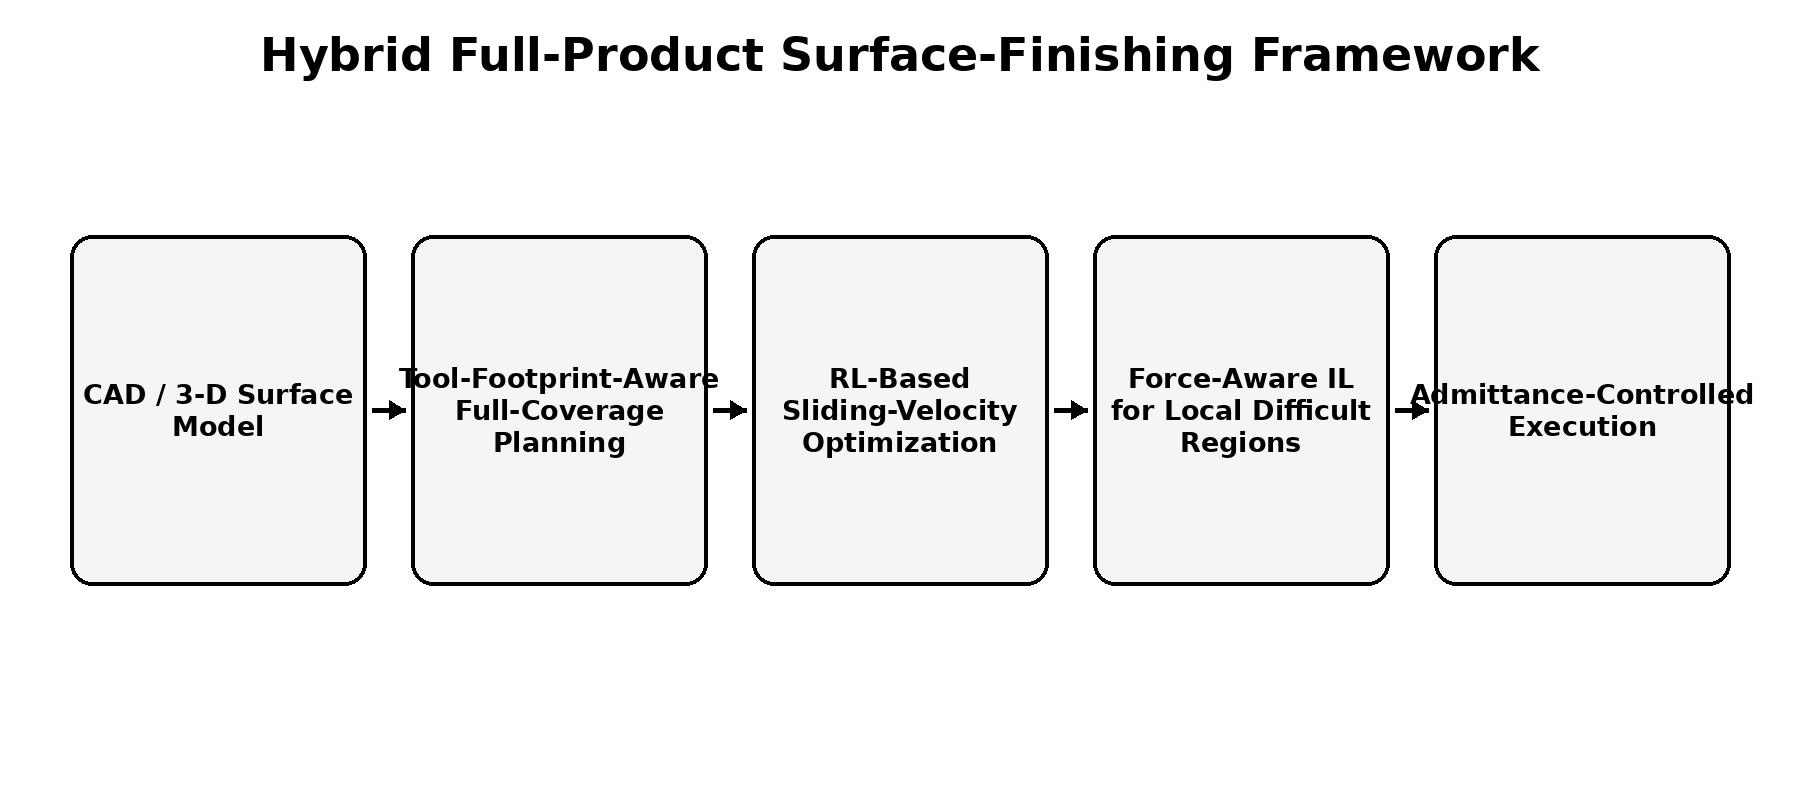
\includegraphics[width=0.98\textwidth]{./1.Introduction/figs/overall_framework.png}
    \caption{Overall structure of the proposed hybrid full-product surface-finishing framework.}
    \label{fig:overall_framework}
\end{figure}

\section{Related Works}
\subsection{Surface Reconstruction and Coverage Planning}
Scan-based robotic surface finishing has progressed from planar projection toward free-form surface reconstruction, segmentation, geodesic planning, and kinematics-aware optimization. Tafuro et al. studied planning from realistic industrial scans and emphasized incomplete reconstruction and abrupt curvature changes~\cite{tafuro2024autonomous}. Schneyer et al. segmented free-form surfaces and selected different finishing-disk contact points to improve access to concave regions~\cite{schneyer2023segmentation}. Gong et al. generated uniform coverage trajectories on equation-free mesh surfaces~\cite{gong2025uniform}, while recent planners exploit redundancy, region decomposition, and task-aware partitioning~\cite{wang2025coverage,pusnik2025region,yu2026fusion}.

These studies show that local feature coverage can be addressed geometrically when the workpiece and tool model are accurate. Nevertheless, every new contact mode may require a new region classifier, contact-point rule, clearance threshold, or trajectory topology. This thesis retains advanced geometric planning as a strong baseline but uses imitation learning where the desired strategy depends jointly on geometry, visual condition, and contact feedback.

\subsection{Material-Removal Optimization and Reinforcement Learning}
Coverage and removal uniformity are distinct. Recent polishing studies jointly consider force, position, and speed~\cite{adaptive2025force}, constant-pressure processing on curved surfaces~\cite{huang2025marble}, or data-driven material-removal estimation~\cite{darowski2025mrr}. Reinforcement learning has also been used to learn abrasive shape transitions or force-responsive finishing skills~\cite{hachimine2023grinding,wang2023adaptive}. In contrast, the proposed RL policy controls only a scalar path-progress rate above a fixed CAD path and admittance controller. This restricted action space is intended to improve safety, interpretability, and sim-to-real transfer.

\subsection{Force-Aware Imitation Learning}
Force-aware imitation learning has rapidly developed for contact-rich tasks. ForceMimic records force-motion demonstrations and predicts hybrid force-position parameters~\cite{liu2025forcemimic}. FoAR fuses RGB and high-frequency force/torque signals with a future-contact predictor~\cite{he2025foar}. DexForce computes force-informed actions from kinesthetic demonstrations~\cite{chen2025dexforce}, and Flow with the Force Field learns compliant flow-matching policies from demonstration-guided simulation data~\cite{li2026flowforce}. These methods establish that force is valuable in contact-rich policy learning, but they also prevent a broad novelty claim based only on force input or output. The contribution of this thesis is instead defined by selective local teaching, a continuous 9-D pose--force action chunk, direct integration with an admittance controller, and full-product coordination with global planning and RL process optimization.

\subsection{Object-Centric and Mask-Guided Policy Learning}
VIOLA constructs object-centric representations from general object proposals generated by a pretrained vision model and uses a transformer policy to attend to task-relevant visual factors~\cite{zhu2023viola}. Mask2Act predicts future masks of task-relevant objects as latent plans from action-free video and uses them to guide policy learning with limited robot action data~\cite{zhang2025mask2act}. Both methods are relevant to polishing, where bright reflections, background texture, and non-target hardware can dominate a conventional image encoder. Chapter~\ref{chap:feature_masking} adapts their ideas to a force-aware polishing policy.

\section{Research Objectives}
The objective is to develop and evaluate a modular framework with the following functions:
\begin{enumerate}
    \item generate a full-coverage path over an entire CAD surface using the effective polishing-tool footprint and overlap ratio;
    \item learn an adaptive sliding-velocity policy that reduces spatial variation of the Preston rate without directly controlling robot joints or the 6-D pose;
    \item learn local pose--force action chunks from expert demonstrations for edges and contact-sensitive regions;
    \item incorporate VIOLA-inspired region tokens and Mask2Act-inspired predictive mask plans into the force-aware IL framework;
    \item validate the complete framework on a guitar-scale object using coverage, removal, force, safety, efficiency, and generalization metrics.
\end{enumerate}

\section{Thesis Organization}
Chapter~2 defines the shared system interfaces and problem formulation. Chapter~3 presents tool-footprint-aware full-coverage path planning. Chapter~4 describes RL-based sliding-velocity optimization. Chapter~5 presents force-aware imitation learning. Chapter~6 proposes the feature-masking architecture. Chapter~7 defines the experimental design, and Chapter~8 concludes the thesis and outlines future work.

\markboth{Related Work}{Related Work}
\chapter{Related Work}
\label{chap:related_work}

\section{Robotic Surface Repair and Polishing}
Robotic surface processing combines task specification, path planning, contact regulation, and process monitoring. Coverage planners reason about workpiece boundaries, tool footprints, reachability, and collision constraints, while polishing controllers regulate contact along curved surfaces~\cite{schneyer2023segmentation,mcgovern2024coverage,mohsin2019path}. Integrated surface-treatment systems demonstrate the value of connecting inspection, planning, and controlled execution~\cite{alt2024robogrind,tafuro2024autonomous}. FAIRE focuses specifically on the division between uncertain defect-dependent treatment and quantitative post-removal blending.
% TODO: Add references on robotic defect repair and blending.

\section{Vision-Based Defect Localization and Geometric Repair Planning}
Vision can identify candidate defect regions and provide geometry for a local path. Such localization answers where a defect appears, but a repair controller also needs a target removal amount and process conditions. These values are especially uncertain when appearance is an incomplete proxy for depth and material response. FAIRE therefore treats visual context as part of an expert policy observation instead of assuming that an image-space region fully specifies the repair.
% TODO: Add verified references on vision-based defect localization for robotic repair.

\section{Imitation Learning for Contact-Rich Manipulation}
Visuomotor imitation policies learn temporally coherent actions from demonstrations~\cite{zhao2023act,chi2025diffusionpolicy}. Contact-rich manipulation adds latent interaction state: similar images and poses can correspond to approach, stable contact, excessive loading, or contact loss. Force-aware methods incorporate wrench observations or force-related actions to reduce this ambiguity~\cite{zhou2024admitdiff,liu2025forcemimic,he2025foar,yang2023momaforce}. FAIRE uses this principle to learn defect-conditioned selective treatment rather than generic trajectory replay.

\section[Force-Aware Motion--Force Demonstration Learning]{Force-Aware Motion--Force\\ Demonstration Learning}
External teaching devices can capture human motion independently of a robot embodiment, while force/torque instrumentation records the accompanying interaction. ForceMimic provides a relevant precedent for force--motion capture in contact-rich tasks~\cite{liu2025forcemimic}. FAIRE retains a handheld device equipped with a six-axis force/torque sensor, VR-to-robot calibration, and synchronized image, pose, orientation, and wrench recording. Its subsystem study compares current-wrench and wrench-history observations and MLP, LSTM, and GRU encoders without claiming novelty for recurrence itself.

\section{Admittance and Compliant Contact Control}
Impedance and admittance control specify compliant relations between motion and interaction force~\cite{hogan1985impedance,villani2008forcecontrol,keemink2018admittance}. Admittance control is appropriate when a policy provides a desired contact force but the robot accepts Cartesian motion references. In FAIRE, desired contact force always denotes a controller-level reference. The controller changes the normal-direction position to track it; the policy output is not a direct actuator force.

\section{Material-Removal Modeling and Tool Influence Functions}
Preston's model relates removal to pressure and relative velocity~\cite{preston1927theory}. Spatial polishing models further require a tool influence function (TIF) describing how contact distributes removal around a tool pose. A usable repair map must combine calibrated process response, normal force, true tool--surface relative velocity, dwell, overlap, and tool geometry. FAIRE introduces this established modeling principle as the bridge from executed IL behavior to a spatial estimate; it does not claim Preston's relation or the TIF concept as new.
% TODO: Add verified references on TIF calibration and spatial material-removal prediction.

\section{Robotic Blending and Coverage Planning}
Coverage planning generates raster, contour, or related paths over a defined region and assigns spacing, overlap, and process conditions~\cite{schneyer2023segmentation,mcgovern2024coverage}. For localized blending, uniform processing with an abrupt boundary is undesirable because it can preserve a step between processed and intact material. FAIRE instead defines a uniform target in a core region and a smoothly decreasing target in a transition band, then plans only the additional removal demanded by their residual map.

\section{Residual Learning for Surface and Process Adaptation}
Residual learning places bounded learned corrections around a nominal controller, limiting the policy's responsibility and preserving an interpretable baseline. Related contact-rich work supports learned reactive or compliance-aware corrections~\cite{hou2025adaptivecompliance,xue2025reactivediffusion}. In FAIRE, residual RL is restricted to the blending stage. Roll and pitch adapt tool orientation, and a feed-velocity residual responds to spatially varying removal demand and contact stability. Neither residual modifies the demonstrated expert IL stroke.

\section{Positioning of FAIRE}
\begin{table}[t]
\centering
\caption{Functional positioning of FAIRE. Entries describe responsibilities rather than claims of algorithmic novelty.}
\label{tab:related_positioning}
\small
\begin{tabularx}{\textwidth}{p{0.22\textwidth}XXX}
\toprule
Component & Input or target & Responsibility & Boundary \\
\midrule
Expert IL & Image, robot state, six-axis wrench history & Infer defect-conditioned selective treatment & Does not produce a quantitative restoration profile \\
Removal model & Actual execution history & Estimate spatial processing/removal produced by IL & Proxy until \(K\) and TIF are calibrated \\
Blending planner & Target and residual-removal maps & Specify local coverage and nominal process conditions & Does not infer original defect severity \\
Admittance & Desired contact force & Adapt normal position to unknown height & Force is a controller-level reference \\
Residual RL & Local blending state and residual demand & Adapt roll, pitch, and tangential feed velocity & Active only during blending \\
\bottomrule
\end{tabularx}
\end{table}

FAIRE is positioned as an integrated system in which IL acts as an expert and model-based blending acts as a structured restoration skill. Its research claim must be evaluated by the staged experiments in Chapter~\ref{chap:experiments}; the present draft reports no positive quantitative result.

\markboth{Problem Formulation and FAIRE Overview}{Problem Formulation and FAIRE Overview}
\chapter{Problem Formulation and FAIRE Overview}
\label{chap:faire_overview}

\section{Surface-Repair Objective}
Let \(\Omega\) denote a bounded local repair workspace on a surface, and let \(q\in\Omega\) denote a point in its local two-dimensional parameterization. The objective is first to remove a visually observed defect selectively and then to obtain a spatial material-removal profile that is uniform around the defect and smoothly connected to the intact surface. The system must avoid excessive force, workspace violation, contact loss, and overprocessing subject to implementation-specific safety limits.

\section{Skill--Expert Problem Formulation}
A geometric skill receives a target region and process parameters and executes them. An expert instead infers appropriate treatment from uncertain evidence. FAIRE assigns the mapping from visual/contact evidence to selective repair behavior to expert IL, while assigning a quantitatively defined residual-removal objective to the blending skill.

\begin{figure}[t]
  \centering
  \fbox{\begin{minipage}[c][0.21\textheight][c]{0.90\textwidth}
    \centering
    \textbf{Geometric skill:}\\
    predefined target \(+\) process parameters \(\rightarrow\) structured execution\\[1.3ex]
    \textbf{Expert IL:}\\
    image \(+\) robot state \(+\) wrench history\\
    \(\rightarrow\) treatment, process intensity, local repetition, and termination
  \end{minipage}}
  \caption{Skill--expert distinction used throughout FAIRE. Termination is a policy responsibility only if the final implementation supports learned continuation or stopping.}
  \label{fig:skill_expert}
\end{figure}

\section{Expert IL for Selective Defect Removal}
The conceptual IL observation is
\begin{equation}
  o_t^{\mathrm{IL}}=\{I_t,s_t,w_{t-K:t}\},
  \label{eq:il_observation}
\end{equation}
where \(I_t\) is the visual observation, \(s_t\) is the current robot/tool state, and \(w_{t-K:t}\) is recent six-axis wrench history. The policy predicts
\begin{equation}
  \pi_{\mathrm{IL}}(o_t^{\mathrm{IL}})
  \rightarrow
  \{x^{\mathrm{ref}}_{t:t+H},
    R^{\mathrm{ref}}_{t:t+H},
    f^{\mathrm{des}}_{t:t+H}\},
  \label{eq:il_policy_overview}
\end{equation}
where \(f^{\mathrm{des}}\in\mathbb{R}^{3}\) is the desired three-axis force trajectory unless the final implementation establishes a different output. The demonstrated tangential feed velocity is preserved:
\begin{equation}
  v_{\mathrm{cmd}}^{\mathrm{IL}}=v_{\mathrm{IL}}.
  \label{eq:preserve_il_velocity}
\end{equation}
Only a deterministic safety governor may reduce or stop IL motion.

\section{Execution-Derived Material-Removal Estimation}
The system logs actual IL execution as
\begin{equation}
  \mathcal{T}_{\mathrm{IL}}
  =
  \{p_t,R_t,w_t,v_{\mathrm{feed},t},\omega_{\mathrm{spindle},t}\}_{t=1}^{T},
  \label{eq:il_execution_log}
\end{equation}
using available measured or estimated values. Commanded pose, measured robot/TCP pose, and estimated contact-point pose are separate quantities. After wrench compensation and contact-frame transformation, this history is converted into a Preston-model-based estimated material-removal map \(\hat h_{\mathrm{IL}}(q)\). Until calibration and metrology validate its units, it is called a removal proxy or relative processing-intensity map.

\section{Target Profile and Residual-Removal Formulation}
The target profile contains a defect-covering core \(\Omega_{\mathrm{core}}\) and an outer transition band \(\Omega_{\mathrm{transition}}\):
\begin{equation}
  h^{*}(q)=
  \begin{cases}
    h_c, & q\in\Omega_{\mathrm{core}},\\
    h_c w(d(q)), & q\in\Omega_{\mathrm{transition}},\\
    0, & \text{otherwise},
  \end{cases}
  \label{eq:target_profile_overview}
\end{equation}
where \(w(d)\) decreases smoothly from one to zero. The required additional removal is
\begin{equation}
  \Delta h(q)=\max\{0,h^{*}(q)-\hat h_{\mathrm{IL}}(q)\}.
  \label{eq:residual_removal_overview}
\end{equation}
Because removal is irreversible, the nonnegative residual cannot compensate for IL over-removal.

\section{CAD-Free Adaptive Blending}
The residual map determines where additional processing is required and provides a quantitative demand for a local raster or contour planner. The planner selects nominal force, tangential feed velocity, overlap, path spacing, and pass count. Admittance control adjusts normal position for unknown height, and residual RL adapts orientation and feed velocity on smooth unseen geometry.

\begin{figure}[t]
  \centering
  \fbox{\begin{minipage}[c][0.31\textheight][c]{0.91\textwidth}
    \centering
    \textbf{VR-calibrated handheld teaching}\\
    \(\downarrow\) synchronized image--pose--orientation--wrench data\\
    \textbf{Expert IL selective repair}\\
    \(\downarrow\) actual execution logging\\
    \textbf{Preston-model-based removal map}\\
    \(\downarrow\) target core/transition profile and residual map\\
    \textbf{Model-based local blending plan}\\
    \(\downarrow\) admittance height adaptation\\
    \(\quad+\) residual roll/pitch and feed-velocity adaptation
  \end{minipage}}
  \caption{End-to-end FAIRE architecture. Residual orientation and velocity policies operate during model-based blending only.}
  \label{fig:faire_architecture}
\end{figure}

\section{Module Responsibilities}
\begin{table}[t]
\centering
\caption{Responsibility allocation in the end-to-end system.}
\label{tab:module_responsibilities}
\small
\begin{tabularx}{\textwidth}{p{0.22\textwidth}XX}
\toprule
Module & Determines & Does not determine \\
\midrule
Expert IL & Defect-dependent motion, force, repetition, and implemented stopping behavior & Post-repair spatial regularization \\
Removal estimator & Spatial effect of the executed process & New material addition or defect semantics \\
Target-profile rule & Desired core depth and transition shape & Robot contact response \\
Blending planner & Coverage geometry and nominal process conditions & Original defect severity \\
Admittance & Normal-direction height correction & Tangential coverage direction \\
Residual RL & Bounded blending-only roll, pitch, and feed-velocity corrections & IL execution or global path topology \\
\bottomrule
\end{tabularx}
\end{table}

\section{Assumptions and Safety Boundary}
The framework assumes a local parameterizable region, smooth continuous surface variation, moderate curvature, a compatible compliant tool, and calibrated process conditions. It does not assume online access to a CAD-derived perfect normal. Any surface normal used as privileged training reward information must remain outside the online observation unless actually measured. Deterministic force, velocity, orientation, workspace, and cumulative-process limits bound both stages. Exact limits are \todoexp{to be determined from the final implementation}.

\markboth{Demonstration Collection}{Demonstration Collection}
\chapter{VR-Calibrated Motion--Force Demonstration Collection}
\label{chap:demonstration_collection}

\section{Teaching-System Purpose}
The teaching system records how an operator interprets and treats a localized defect, including the motion pattern, tangential feed velocity, desired contact behavior, and local repetition. FAIRE retains a handheld teaching device equipped with a six-axis force/torque sensor and tracked in a virtual-reality (VR) coordinate frame. An RGB camera supplies visual task context. Image, position, orientation, and wrench streams are synchronized so that each action can be associated with the corresponding defect appearance and interaction history.

\section{Coordinate Frames and Pose Transfer}
Let \(B\), \(V\), \(T\), \(S\), \(E\), and \(C\) denote the robot base, VR tracking, tracker, force/torque sensor, TCP/tool, and contact-point frames. The demonstrated TCP pose in the robot base is
\begin{equation}
  {}^{B}\!T_{E}^{\mathrm{demo}}(t)
  =
  {}^{B}\!T_{V}\,
  {}^{V}\!T_{T}(t)\,
  {}^{T}\!T_{E}.
  \label{eq:demo_transfer}
\end{equation}
The transform \({}^{B}\!T_V\) is obtained from VR-to-robot calibration, \({}^{V}\!T_T(t)\) is tracked over time, and \({}^{T}\!T_E\) is the fixed tracker-to-tool transform. Calibration observations, estimation method, and validation residuals are \todoexp{to be determined from the final implementation}.

\begin{figure}[t]
  \centering
  \fbox{\begin{minipage}[c][0.21\textheight][c]{0.90\textwidth}
    \centering
    Robot base \(B\) \(\leftarrow\) VR frame \(V\) \(\leftarrow\) tracker \(T\)\\
    \(\downarrow\) tracker-to-tool calibration\\
    TCP/tool frame \(E\) \(\rightarrow\) contact-point frame \(C\)\\[1ex]
    synchronized \(I_t,\ p_t,\ R_t,\ w_t,\) and timestamps
  \end{minipage}}
  \caption{Coordinate chain for VR-to-robot demonstration transfer and contact-point representation. Numerical calibration results and the final apparatus drawing remain TBD.}
  \label{fig:demo_transfer}
\end{figure}

\section[Wrench Processing and Contact-Point Representation]{Wrench Processing and Contact-Point\\ Representation}
The sensor produces a six-axis wrench
\begin{equation}
  w_t^S=[F_x,F_y,F_z,\tau_x,\tau_y,\tau_z]_t^{S}.
\end{equation}
The usable wrench requires bias removal, gravity and tool-load compensation, filtering, and transformation to a declared contact or tool frame. When the reference point changes, the spatial wrench transform must account for the associated moment arm; rotating force components alone is insufficient. The same sign convention and reference point must be used in demonstrations, policy observations, force control, removal estimation, and evaluation.

The contact-point pose differs from the measured TCP pose by the TCP-to-contact transform:
\begin{equation}
  {}^{B}\!T_C(t)={}^B\!T_E(t)\,{}^E\!T_C.
  \label{eq:contact_pose}
\end{equation}
The offset \({}^E\!T_C\) depends on pad/tool geometry and may vary with compliant deformation. The final implementation must state whether the contact pose is measured, estimated from a rigid offset, or corrected by a compliance model. Unverified deformation compensation is not assumed.

\section{Synchronization and Dataset Construction}
An episode is stored conceptually as
\begin{equation}
  D_i=\{I_t,p_t,R_t,w_t,v_{\mathrm{feed},t},m_t\}_{t=1}^{T_i},
  \label{eq:demonstration_dataset}
\end{equation}
where \(m_t\) denotes available metadata or event labels. Each stream requires timestamps. The synchronization method must report acquisition rates, clock convention, interpolation or resampling, maximum accepted skew, missing-sample handling, and any measured delay. These values are \todoexp{TBD}. Misalignment is particularly harmful because it pairs visual and pose context with a wrench produced at another contact phase.

\section{Episode Segmentation and Training Windows}
Episodes should separate approach, selective processing, local repetition, and release when these phases can be identified reliably. A training sample at time \(t\) contains the current image and robot state, the wrench history \(w_{t-K:t}\), and a future reference horizon through \(t+H\). Boundary handling, padding masks, stride, \(K\), and \(H\) are \todoexp{to be determined from the final implementation}.

Dataset partitions are made at the episode, defect, or specimen-trial level. Adjacent windows from one episode must not be split across training and evaluation because that would leak nearly identical temporal context. Normalization statistics and augmentation are fitted using training data only.

\section{Demonstration Quality, Metadata, and Safety}
Episodes are rejected or labeled if they contain tracker loss, sensor saturation, timestamp discontinuity, accidental collision, unsafe load, or missing images. Transformed trajectories must pass reachability, collision, workspace, velocity, and force checks before robot execution. Calibration establishes coordinate correspondence but does not guarantee safe motion.

Required records include operator and specimen identifiers, defect preparation, material and coating, tool and abrasive state, spindle setting if applicable, sensor zeroing, calibration version, contact threshold, start pose, processing annotations, and safety events. Appendix~\ref{chap:appendix} provides the completion checklist.

\markboth{Force-Aware Expert Imitation}{Force-Aware Expert Imitation}
\chapter{Force-Aware Expert Imitation for Selective Defect Removal}
\label{chap:force_il}

\section{Expert Repair Objective}
The expert IL module determines how and to what extent a visually observed defect should be selectively removed from visual context and interaction history. It learns the operator's defect-conditioned local motion pattern, desired contact force, demonstrated tangential feed-velocity profile, and repeated visits. It is not described as an explicit detector, and it is not reduced to replaying a path whose treatment parameters are already known.

\section{Visual, Robot-State, and Wrench-History Observation}
The policy observation follows Eq.~\eqref{eq:il_observation}. Separate encoders compute
\begin{align}
  z_t^I &= f_I(I_t),&
  z_t^s &= f_s(s_t),&
  z_t^w &= \operatorname{GRU}(w_{t-K:t}),
  \label{eq:policy_encoders}
\end{align}
and a fusion module produces \(z_t=\operatorname{Fusion}(z_t^I,z_t^s,z_t^w)\). The force branch uses six-axis wrench history as a policy observation. Tangential forces and moments can distinguish partial contact, tool tilt, and unstable interaction that a scalar normal force may conceal. The image encoder, robot-state fields, dimensions, GRU hidden size, and fusion design are \todoexp{TBD}.

\begin{figure}[t]
  \centering
  \fbox{\begin{minipage}[c][0.22\textheight][c]{0.90\textwidth}
    \centering
    \(I_t\rightarrow\) visual encoder \(\rightarrow z_t^I\)\\
    \(s_t\rightarrow\) robot-state encoder \(\rightarrow z_t^s\)\\
    \(w_{t-K:t}\rightarrow\) GRU wrench-history encoder \(\rightarrow z_t^w\)\\[1ex]
    fused representation \(\rightarrow\)
    \(\{x^{\mathrm{ref}}_{t:t+H},R^{\mathrm{ref}}_{t:t+H},
    f^{\mathrm{des}}_{t:t+H}\}\)
  \end{minipage}}
  \caption{Force-aware expert imitation architecture. The desired three-axis force trajectory is a controller-level reference; exact network dimensions remain TBD.}
  \label{fig:force_history_policy}
\end{figure}

\section{Motion--Force Trajectory Prediction}
The short-horizon prediction is
\begin{equation}
  \pi_{\mathrm{IL}}(z_t)
  \rightarrow
  \left\{
    x^{\mathrm{ref}}_{t:t+H},
    R^{\mathrm{ref}}_{t:t+H},
    f^{\mathrm{des}}_{t:t+H}
  \right\}.
  \label{eq:motion_force_prediction}
\end{equation}
Position and orientation describe demonstrated motion. The desired three-axis force trajectory describes the contact reference to be realized compliantly. Overlapping-horizon selection, temporal ensembling, prediction frequency, and orientation parameterization are \todoexp{to be determined from the final implementation}.

\section{Supervised Learning Objective}
A conceptual multitask objective is
\begin{equation}
  \mathcal{L}_{\mathrm{IL}}
  =
  \lambda_x\mathcal{L}_{x}
  +\lambda_R\mathcal{L}_{R}
  +\lambda_f\mathcal{L}_{f},
  \label{eq:imitation_loss}
\end{equation}
where the terms penalize position, rotation, and desired-force trajectory error. A rotation-aware loss is required for the selected orientation representation. Loss definitions, weights, normalization, padding masks, optimizer, schedule, batch size, training duration, seeds, and checkpoint selection remain \todoexp{TBD}. Equation~\eqref{eq:imitation_loss} does not imply a finalized network or training recipe.

\section{Why Force History Is Required}
An instantaneous wrench may be similar during contact establishment, stable processing, or recovery from overload. A history window provides contact trend, persistence, and phase information. The GRU is separated from the visual and robot-state encoders so that current-wrench, flattened-history, LSTM, and GRU variants can be compared while retaining the same policy output and controller. These comparisons test whether temporal contact context supports expert imitation; they do not claim that the GRU is novel.

\section{Why Geometric Localization Alone Is Insufficient}
A localized region describes where processing is allowed or likely needed, but not the correct intensity at each point. Similar image-space defects may demand different force profiles or repetition, and the interaction history may reveal whether a local pass is effective. The expert policy therefore learns a conditional treatment rather than receiving a complete geometric recipe. Experiment~I in Chapter~\ref{chap:experiments} tests this necessity against fixed geometric/ROI processing and vision-only variants.

\section{Admittance-Based Desired-Force Execution}
\label{sec:admittance_il}
The desired contact force is tracked through admittance dynamics:
\begin{equation}
  M_d\Delta\ddot p_t+
  D_d\Delta\dot p_t+
  K_d\Delta p_t
  =
  f_t^{\mathrm{meas}}-f_t^{\mathrm{des}},
  \label{eq:admittance_il}
\end{equation}
with command composition
\begin{equation}
  p_t^{\mathrm{cmd}}=p_t^{\mathrm{ref}}+\Delta p_t^{\mathrm{adm}}.
  \label{eq:il_position_command}
\end{equation}
The selected controlled axes and sign convention must be stated. The discrete update, virtual parameters, filtering, saturation, contact-state reset, and robot interface are \todoexp{TBD}. The learned force is never interpreted as a direct actuator command.

\section{Preservation of Demonstrated Feed Velocity}
During expert IL, the commanded tangential feed velocity equals the demonstrated IL velocity as stated in Eq.~\eqref{eq:preserve_il_velocity}. A residual velocity policy is not active because it would alter the operator strategy whose defect-dependent behavior is being reproduced. A deterministic governor may only reduce or stop motion when excessive force, contact loss, workspace violation, command discontinuity, or another declared safety condition is detected.

\section{Local Repetition and Termination}
Repeated processing can appear implicitly in the predicted pose sequence or be represented by an explicit continuation decision. The current repository does not establish a learned stopping output. Accordingly, continuation and termination are \todoexp{to be determined from the final implementation}. If execution uses a fixed horizon, operator stop, visual threshold, or explicit rule, that mechanism must be reported and evaluated without being described as learned termination.

\section{Online Execution and Safety Governor}
At each update, the system preprocesses the image, robot state, and compensated wrench; updates the six-axis history; predicts the reference horizon; selects the current pose and desired-force references; integrates the admittance correction; and applies deterministic safety bounds. The actual measured TCP pose, estimated contact pose, compensated wrench, tangential feed velocity, spindle speed if available, commanded references, contact state, and safety events are logged for Chapter~\ref{chap:removal_estimation}. Residual RL remains disabled throughout this stage.

\markboth{Material-Removal Estimation}{Material-Removal Estimation}
\chapter{Execution-Derived Material-Removal Estimation}
\label{chap:removal_estimation}

\section{Process-Data Logging during IL Execution}
Removal estimation uses the process that the robot actually executed, not the policy command alone. For every sample, the log distinguishes commanded TCP pose, measured robot/TCP pose, and estimated contact-point pose. It also records the raw and processed wrench, measured tangential feed velocity, spindle angular speed when available, contact state, timestamps, and safety interventions. The execution record is \(\mathcal{T}_{\mathrm{IL}}\) in Eq.~\eqref{eq:il_execution_log}.

Commanded pose is retained for controller analysis but is not substituted for contact location when following error or compliance is significant. The mapping from TCP to contact point uses the calibrated offset and pad/tool geometry from Eq.~\eqref{eq:contact_pose}. Any compliance-related contact-location correction is \todoexp{TBD}.

\section{Contact Frame and Normal-Force Computation}
Let \(f_t\) be the compensated force expressed in a common frame, and let \(n_t\) be the unit tool or estimated surface normal used by the removal model. Normal force is the projection
\begin{equation}
  F_n(t)=f_t^\mathsf{T}n_t,
  \label{eq:normal_force_projection}
\end{equation}
with sign chosen so that compressive contact is positive. Sensor \(F_z\) is not assumed to be the normal force unless the sensor frame is verified to be aligned with \(n_t\).

The online system does not assume access to a perfect CAD normal. During IL map construction, \(n_t\) may be obtained from the measured tool orientation under an aligned-tool assumption, from a verified local estimator, or from another implemented source. The chosen method and its uncertainty are \todoexp{to be determined from the final implementation}. Samples below a validated contact threshold are excluded from material removal.

\section{Preston-Based Spatial Removal Model}
A discrete spatial model is
\begin{equation}
  \hat h_{\mathrm{IL}}(q)
  =
  \sum_{t=1}^{T}
  K\,F_n(t)\,
  G(q;p_t,R_t)\,
  v_{\mathrm{rel}}(q,t)\,\Delta t,
  \label{eq:preston_spatial}
\end{equation}
where \(K\) is the calibrated Preston coefficient, \(G\) is a normalized TIF centered and oriented by the contact pose, and \(v_{\mathrm{rel}}(q,t)\) is the magnitude of true tool--surface relative velocity at \(q\). The model accumulates overlapping dwell and repeated passes.

Tangential robot feed velocity and true relative sliding are distinct. If the pad rotates, spindle motion may dominate \(v_{\mathrm{rel}}\), while feed changes dwell and the path of the influence footprint. The final implementation must calculate \(v_{\mathrm{rel}}\) from the available kinematics and tool geometry rather than replacing it automatically with \(v_{\mathrm{feed}}\).

\section{Tool Influence Function}
The TIF \(G(q;p_t,R_t)\) describes the normalized spatial distribution of removal around a tool pose:
\begin{equation}
  G(q;p_t,R_t)\geq 0,
  \qquad
  \int_{\Omega}G(q;p_t,R_t)\,dq=1
  \label{eq:tif_normalization}
\end{equation}
over a sufficiently large local domain. Its shape may depend on pad geometry, compliance, force, tilt, spindle speed, abrasive state, and material. FAIRE will use the simplest calibrated parameterization supported by measurements; a Gaussian, measured lookup map, or another shape is not assumed before calibration.

\section{Calibration and Metrology}
Controlled polishing tests will vary one declared factor at a time over safe operating ranges and measure the resulting removal. Calibration must cover force dependence, relative-velocity or dwell dependence, spatial TIF shape, and repeated-pass accumulation. The Preston coefficient \(K\) is fitted only after defining units and the specific tool--abrasive--material condition.

Removal maps will be measured by a verified method such as profilometry, confocal measurement, laser measurement, or another metrology system whose resolution and registration are documented. \todoexp{Select the metrology instrument, calibration specimens, factor levels, fitting procedure, and validation split.} The validation compares predicted and measured depth maps on held-out process conditions or specimens. Until this is complete, \(\hat h\) is reported only as a removal proxy or relative processing-intensity map.

\section{Estimated IL Removal Map}
The logged trajectory is rasterized in the local repair coordinates, and each valid contact sample contributes the shifted and oriented TIF weighted by normal force, relative velocity, and sample duration. Registration between robot coordinates and the measured surface map must be reported. Map resolution should be fine enough to represent the TIF without implying precision beyond the metrology system.

\begin{figure}[t]
  \centering
  \fbox{\begin{minipage}[c][0.22\textheight][c]{0.90\textwidth}
    \centering
    actual IL contact poses \(+\) compensated normal force\\
    \(+\) true relative velocity \(+\) calibrated \(K,G\)\\
    \(\downarrow\) spatial accumulation\\
    \(\hat h_{\mathrm{IL}}(q)\)
    \(\quad\) compared with \(\quad h^*(q)\)\\
    \(\downarrow\) \(\Delta h(q)=\max(0,h^*-\hat h_{\mathrm{IL}})\)
  \end{minipage}}
  \caption{Conceptual construction of the execution-derived removal map and residual-removal map. Experimental maps will replace the placeholder after calibration and metrology.}
  \label{fig:removal_and_residual_maps}
\end{figure}

\section{Target Core and Transition Profiles}
The target profile is defined by Eq.~\eqref{eq:target_profile_overview}. The core contains the defect and is regularized toward a constant \(h_c\). The transition band connects this plateau to zero additional removal on the intact surface. A smooth weight can satisfy
\begin{equation}
  w(0)=1,\quad w(D)=0,\quad
  w'(0)=w'(D)=0,\quad 0\leq w(d)\leq 1,
  \label{eq:transition_conditions}
\end{equation}
where \(d\in[0,D]\) measures outward distance through a band of width \(D\). The final taper function and definition of distance are \todoexp{TBD}.

\begin{figure}[t]
  \centering
  \fbox{\begin{minipage}[c][0.21\textheight][c]{0.90\textwidth}
    \centering
    \(\underbrace{\rule{0.22\textwidth}{1.2pt}}_{\Omega_{\mathrm{core}}:\ h_c}\)
    \(\;\searrow\;\)
    \(\underbrace{\text{smooth decay to }0}_{\Omega_{\mathrm{transition}}}\)\\[1.5ex]
    uniformize the inner repair region \(\rightarrow\)
    blend gradually into the intact surface
  \end{minipage}}
  \caption{Target removal profile with a uniform core and a smoothly decaying transition band.}
  \label{fig:target_profile}
\end{figure}

The selection of \(h_c\) must be explicit and conservative. Candidate rules include a measured defect-depth estimate, a robust percentile or plateau of the IL removal map, or a process-specific target under a coating-thickness safety bound. A noisy maximum is not used without statistical and physical justification. The final rule is \todoexp{TBD}.

\section{Residual-Removal Map}
The residual map in Eq.~\eqref{eq:residual_removal_overview} assigns minimal additional processing where IL has already reached the target and additional removal where it has not. It also adds the controlled transition processing needed to connect the repaired core to the intact surface. An uncertainty margin or conservative dead band may be required to prevent model error from causing over-removal; its definition is \todoexp{TBD}.

\section{Model Limitations and Uncertainty}
Preston behavior may deviate from linearity because of pad wear, abrasive loading, temperature, saturation, compliance, changing contact area, material heterogeneity, and tool tilt. A fixed TIF approximates a process that may vary with force and orientation. Pose, normal, clock, and metrology registration errors propagate into the spatial map. Most importantly, the model can request additional removal but cannot add material after IL over-removes. These limitations motivate conservative targets, held-out validation, uncertainty reporting, and eventual post-pass inspection.

\markboth{CAD-Free Model-Based Blending}{CAD-Free Model-Based Blending}
\chapter{CAD-Free Model-Based Blending with Residual RL}
\label{chap:blending}

\section{Blending Objective}
The blending stage converts the residual-removal map into structured additional processing. Its objective is to reduce residual error in the core, follow the decaying transition target, preserve intact surroundings, and maintain stable contact. It is a model-based restoration skill: the spatial target and process demand have already been defined by Chapter~\ref{chap:removal_estimation}.

\section{Local Coverage-Path Generation}
The planner generates a local two-dimensional raster or contour path over cells where \(\Delta h(q)\) exceeds a declared threshold. It does not require a complete CAD model or full 3D reconstruction. The local parameterization provides coverage direction and spatial indexing; unknown height is handled by admittance, and moderate orientation variation is handled by residual RL.

Path topology, boundary offset, turning strategy, and collision/reachability checks are \todoexp{TBD}. The planned scope is limited to local, smooth, continuously varying surfaces without sharp edges, steps, grooves, or discontinuities.

\section[Nominal Force, Velocity, Overlap, and Pass Planning]{Nominal Force, Velocity, Overlap,\\ and Pass Planning}
Using the calibrated process model, the planner assigns nominal desired contact force \(f_{\mathrm{nom}}^{\mathrm{des}}\), tangential feed velocity \(v_{\mathrm{nom}}(q)\), path spacing, overlap, and pass count. These quantities should be chosen together because they jointly determine dwell and accumulated removal. A conservative optimizer or rule-based inversion of Eq.~\eqref{eq:preston_spatial} may be used; the implemented method is \todoexp{TBD}.

\section{Admittance-Based Surface-Height Adaptation}
The planner produces nominal Cartesian position \(p_{\mathrm{nom}}\). Admittance control changes its normal component:
\begin{equation}
  p_{\mathrm{cmd}}=p_{\mathrm{nom}}+\Delta p_{\mathrm{adm}},
  \label{eq:blending_admittance}
\end{equation}
so that unknown surface-height variation is accommodated while tracking the desired contact force. The desired contact force remains a controller-level reference. Tangential coverage direction is not generated by admittance.

\section{Residual Tool-Orientation Adaptation}
During blending only, bounded roll and pitch corrections adapt the tool to smooth unseen curvature:
\begin{equation}
  R_{\mathrm{cmd}}
  =
  R_{\mathrm{nom}}
  \operatorname{Exp}\!\left(
    [\Delta\phi_t,\Delta\theta_t,0]_\times
  \right).
  \label{eq:orientation_residual}
\end{equation}
Yaw and coverage direction remain the planner's responsibility unless the final implementation establishes otherwise. The policy must not assume online access to a CAD-derived or perfect surface normal. A simulated normal may be used as privileged reward information during training only if that separation is stated.

\section[Residual-Removal-Aware Feed-Velocity Adaptation]{Residual-Removal-Aware Feed-Velocity\\ Adaptation}
The velocity command is
\begin{equation}
  v_{\mathrm{cmd}}
  =
  \operatorname{clip}
  \left(v_{\mathrm{nom}}(q_t)+\Delta v_t,
  v_{\min},v_{\max}\right).
  \label{eq:velocity_residual}
\end{equation}
The objective is to achieve spatially varying target removal at the desired locations. The policy should slow where residual demand is large, move faster where little removal remains, reduce unnecessary processing near target completion, and slow when force, contact, or orientation becomes unstable. Feed velocity is not called true sliding velocity; the latter is reserved for actual tool--surface relative motion in the removal model.

\section{Residual Policy Observation, Action, and Reward}
The residual action is
\begin{equation}
  \Delta a_t^{\mathrm{RL}}
  =
  [\Delta\phi_t,\Delta\theta_t,\Delta v_t]^\mathsf{T}.
  \label{eq:residual_action}
\end{equation}
A conceptual observation may include local residual-removal demand, six-axis wrench, force-tracking error, current orientation, current and nominal feed velocity, and local path state:
\begin{equation}
  o_t^{\mathrm{RL}}
  =
  [\Delta h_{\mathrm{local}},F_x,F_y,F_z,\tau_x,\tau_y,\tau_z,
  e_F,R_t,v_t,v_{\mathrm{nom}},\xi_t].
  \label{eq:residual_observation}
\end{equation}
This is not an implemented state specification. \todoexp{Finalize the RL observation, normalization, state estimator, algorithm, network, and update rate.}

A conceptual reward may penalize residual-removal error, force-tracking error, tangential wrench, action magnitude, action change, contact loss, and safety violation:
\begin{equation}
  r_t =
  -c_h e_h
  -c_F e_F^2
  -c_w\|w_t^{\mathrm{tan}}\|^2
  -c_a\|\Delta a_t^{\mathrm{RL}}\|^2
  -c_s
  -c_{\mathrm{safety}}.
  \label{eq:conceptual_rl_reward}
\end{equation}
Terms, weights, temporal credit assignment, privileged signals, and termination are \todoexp{TBD}; Eq.~\eqref{eq:conceptual_rl_reward} is only a design envelope.

\begin{figure}[t]
  \centering
  \fbox{\begin{minipage}[c][0.23\textheight][c]{0.90\textwidth}
    \centering
    local 2D nominal coverage path\\
    \(+\ \Delta p_{\mathrm{adm}}\) for surface height\\
    \(+\ [\Delta\phi,\Delta\theta]\) for smooth orientation variation\\
    \(+\ \Delta v\) for residual-removal-aware tangential feed velocity\\
    \(\downarrow\) final bounded Cartesian command
  \end{minipage}}
  \caption{Blending command composition. The residual policies modify model-based blending and never correct the demonstrated IL trajectory.}
  \label{fig:blending_command}
\end{figure}

\section{Interaction between Orientation and Velocity Policies}
Orientation changes contact distribution and measured wrench, while velocity changes dwell, force transients, and removal accumulation. Their coupled effects require a common observation convention, compatible update rates, and final arbitration by safety limits. Experiment~V compares nominal execution, classical moment-based orientation adaptation, orientation-only residual RL, and the full orientation--velocity residual. Separate and joint policies remain \todoexp{to be determined from the final implementation}.

\section{Iterative Removal-Map Update and Replanning}
After blending pass \(k\), the estimated increment can update the accumulated map:
\begin{align}
  \hat h_{k+1}(q)
  &=\hat h_k(q)+\Delta\hat h_{\mathrm{blend},k}(q),\\
  \Delta h_{k+1}(q)
  &=\max\{0,h^*(q)-\hat h_{k+1}(q)\}.
  \label{eq:iterative_update}
\end{align}
This defines the loop \emph{Plan \(\rightarrow\) Execute \(\rightarrow\) Update Removal Map \(\rightarrow\) Replan}. \todoexp{Iterative replanning is a planned extension unless verified in the final implementation}; it must not be reported as completed before that verification.

\section[Safety Limits and Expected Failure Modes]{Safety Limits and Expected\\ Failure Modes}
Actions are clipped before command composition. Deterministic limits cover normal and tangential force, moments, feed velocity, orientation correction, correction rate, admittance displacement, workspace, contact loss, cumulative predicted removal, and emergency stop. Expected failures include TIF mismatch, incorrect residual demand, policy saturation, oscillatory orientation or velocity, contact loss, conflict between residual channels, and extrapolation beyond trained curvature. Interventions and saturation frequency are reported as outcomes rather than silently discarded.

\markboth{Experimental Evaluation}{Experimental Evaluation}
\chapter{Experimental Evaluation}
\label{chap:experiments}

\section{Research Questions and Evaluation Strategy}
The evaluation follows RQ1--RQ4 from Chapter~\ref{chap:introduction} through six staged experiments. Each stage isolates one responsibility before the end-to-end comparison: the need for expert treatment, force-aware representation, removal-model validity, blending contribution, residual adaptation on unseen geometry, and complete repair progression. All numerical fields remain blank until supported by traceable logs and metrology.

\section{Robot, Tool, Sensor, Camera, and Specimens}
The experimental system requires a robot with a Cartesian command interface, a polishing or repair tool, a six-axis force/torque sensor, a visual sensor, and specimens containing reproducible localized defects. The robot, tool, sensor, camera, spindle, abrasive, material, coating, and metrology hardware are \todoexp{to be determined from the final implementation}.

Specimens should cover smooth flat, convex, and concave geometries within a declared curvature range. Sharp edges and discontinuities are excluded. Defect variations may include severity, depth, width, local nonuniformity, required repetition, or removal difficulty only when those conditions can be produced and measured reliably.

\section{Dataset and Train/Validation/Test Splits}
Demonstration windows are split by episode, defect, or specimen rather than by adjacent timestamps. Model-selection trials are separated from final tests. For geometry generalization, RL training surfaces may include flat and selected convex/concave radii, while test surfaces use previously unseen smooth curvature values or combinations. Material, tool, abrasive, and process conditions remain fixed during the geometry study unless cross-material generalization is explicitly evaluated.

Dataset size, split ratios, defect distribution, surface assignments, and seed count are \todoexp{TBD}. The split manifest and preprocessing statistics will be stored with the reproducibility records.

\section{Experiment I: Necessity of Expert Imitation}
Experiment~I tests whether localization plus a predefined skill determines sufficient treatment. The planned comparison includes a geometric/ROI path with a fixed motion--force recipe, vision-only IL, vision--force IL, and full force-history IL. Conditions should include visually similar regions that require measurably different process intensity, repetition, or stopping behavior.

Metrics include defect-removal ratio, task success, collateral removal outside the defect, force-tracking error, pass or repetition count, termination error when defined, and task time. The defect-removal and termination metrics require explicit pre/post measurements and reference criteria before use.

\begin{table}[t]
\centering
\caption{Planned expert IL baseline comparison. Blank entries await experimental results.}
\label{tab:expert_il_baselines}
\small
\begin{tabularx}{\textwidth}{p{0.25\textwidth}XXXX}
\toprule
Method & \makecell{Defect\\removal} & \makecell{Collateral\\removal} & \makecell{Repetition/\\termination} & \makecell{Task\\time} \\
\midrule
Geometric/ROI fixed recipe & & & & \\
Vision-only IL & & & & \\
Vision--force IL & & & & \\
Full wrench-history IL & & & & \\
\bottomrule
\end{tabularx}
\end{table}

\section{Experiment II: Force-Aware IL Representation}
Experiment~II provides subsystem evidence for RQ1. Action-interface comparisons include pose only, force observation without desired-force output, fixed-force admittance, phase-based force, one-step desired force, and horizon desired-force trajectory. Observation/encoder comparisons include current wrench versus wrench history and MLP, LSTM, and GRU variants. All methods in each subcomparison retain the same data split, policy backbone where applicable, controller, and IL-stage velocity rule.

\begin{sidewaystable}[p]
\centering
\caption{Planned force-aware IL ablations. Blank entries await experimental results.}
\label{tab:force_il_ablation}
\scriptsize
\resizebox{\textheight}{!}{%
\begin{tabular}{lllccccc}
\toprule
Variant & Force observation & Policy force output & Force RMSE & Contact loss & Defect removal & Collateral removal & Success \\
\midrule
Pose only & None & None & & & & & \\
Force observation, pose output & Current/history & None & & & & & \\
Fixed-force admittance & History & Fixed reference & & & & & \\
Phase-based force & History & Phase reference & & & & & \\
One-step desired force & History & One step & & & & & \\
Horizon desired-force trajectory & History & Short horizon & & & & & \\
Current-wrench MLP & Current & Short horizon & & & & & \\
Wrench-history MLP & History & Short horizon & & & & & \\
Wrench-history LSTM & History & Short horizon & & & & & \\
Wrench-history GRU & History & Short horizon & & & & & \\
\bottomrule
\end{tabular}}
\end{sidewaystable}
\clearpage

\section{Experiment III: Removal-Model Calibration and Validation}
Controlled tests calibrate \(K\) and \(G\), verify force and velocity/dwell dependence, and evaluate repeated-pass accumulation. Predicted maps are registered to measured maps obtained with the selected metrology system. Training and validation process conditions or specimens are separated.

Depth RMSE is defined after registration as
\begin{equation}
  \operatorname{RMSE}_h
  =
  \sqrt{\frac{1}{|\mathcal{Q}|}
  \sum_{q\in\mathcal{Q}}
  \bigl(\hat h(q)-h_{\mathrm{meas}}(q)\bigr)^2},
  \label{eq:depth_rmse}
\end{equation}
where \(\mathcal{Q}\) is the declared valid measurement set. Spatial correlation, peak and mean removal error, profile error, map similarity, and repeatability are included only after their registration, masking, and aggregation procedures are specified.

\begin{table}[t]
\centering
\caption{Planned removal-model calibration and validation results.}
\label{tab:removal_calibration}
\scriptsize
\begin{tabularx}{\textwidth}{p{0.25\textwidth}XXXXX}
\toprule
Condition & \makecell{Depth\\RMSE} & Correlation & \makecell{Peak\\error} & \makecell{Mean\\error} & \makecell{Repeat-\\ability} \\
\midrule
Force dependence & & & & & \\
Velocity/dwell dependence & & & & & \\
Repeated-pass accumulation & & & & & \\
Held-out map validation & & & & & \\
\bottomrule
\end{tabularx}
\end{table}

\section{Experiment IV: Residual-Removal-Based Blending}
Experiment~IV compares IL only, IL followed by fixed uniform surrounding processing, and IL followed by model-based residual-removal blending. It evaluates whether the proposed target regularizes the core and produces a smooth transition without unnecessary overprocessing.

Core uniformity is reported using a stated dispersion measure over \(\Omega_{\mathrm{core}}\). Residual-removal RMSE compares achieved and target profiles. Transition-profile error is measured only inside \(\Omega_{\mathrm{transition}}\), and boundary slope or gradient is computed using a declared spatial derivative and sampling method. Surface roughness, gloss, haze, or another appearance metric is reported only if a verified instrument or controlled protocol is available.

\begin{table}[t]
\centering
\caption{Planned comparison of IL-only repair and blending strategies.}
\label{tab:blending_ablation}
\scriptsize
\begin{tabularx}{\textwidth}{p{0.26\textwidth}XXXXX}
\toprule
Method & \makecell{Core\\uniformity} & \makecell{Residual\\RMSE} & \makecell{Transition\\error} & \makecell{Over-\\processing} & Appearance \\
\midrule
IL only & & & & & \\
IL + uniform surrounding process & & & & & \\
IL + residual-removal blending & & & & & \\
\bottomrule
\end{tabularx}
\end{table}

\section{Experiment V: Residual RL on Unseen Surface Geometries}
The residual study compares fixed orientation with nominal model velocity, classical moment-based orientation adaptation with nominal velocity, orientation-only residual RL, and full residual orientation--velocity RL. Training and test geometries are disjoint. A classical moment-based method is included only after its gains, frames, and saturation rules are specified.

Normal-force RMSE uses the projected force from Eq.~\eqref{eq:normal_force_projection}. Other metrics include contact-loss rate, tangential-force magnitude, \(\tau_x/\tau_y\), orientation smoothness, residual-removal error, core uniformity, transition error, task time, safety interventions, and policy saturation frequency.

\begin{sidewaystable}[p]
\centering
\caption{Planned residual RL ablation on unseen smooth surface geometries.}
\label{tab:residual_rl_ablation}
\scriptsize
\resizebox{\textheight}{!}{%
\begin{tabular}{lcccccccc}
\toprule
Method & Force RMSE & Contact loss & Tangential force & Orientation smoothness & Removal error & Task time & Interventions & Saturation \\
\midrule
Fixed orientation + nominal velocity & & & & & & & & \\
Moment-based orientation + nominal velocity & & & & & & & & \\
Orientation-only residual RL & & & & & & & & \\
Residual orientation + velocity RL & & & & & & & & \\
\bottomrule
\end{tabular}}
\end{sidewaystable}
\clearpage

\section{Experiment VI: End-to-End Surface Repair}
End-to-end evaluation records the surface before repair, after IL selective removal, and after model-based blending. The intended analysis asks whether IL removes the defect selectively, whether IL-only removal remains spatially nonuniform, and whether blending brings the core and transition closer to the declared target. These are hypotheses, not current findings.

\begin{table}[t]
\centering
\caption{Planned end-to-end results at each repair stage.}
\label{tab:end_to_end}
\scriptsize
\begin{tabularx}{\textwidth}{p{0.24\textwidth}XXXXX}
\toprule
Stage & \makecell{Defect\\measure} & \makecell{Core\\uniformity} & \makecell{Transition\\error} & \makecell{Collateral\\removal} & Appearance \\
\midrule
Before repair & & & & & \\
After expert IL & & & & & \\
After model-based blending & & & & & \\
\bottomrule
\end{tabularx}
\end{table}

\begin{figure}[t]
  \centering
  \fbox{\begin{minipage}[c][0.20\textheight][c]{0.90\textwidth}
    \centering
    before repair \(\mid\) after expert IL \(\mid\) after blending\\[1ex]
    registered appearance, surface profile, and removal-map panels\\
    \todoexp{to be populated from experimental results}
  \end{minipage}}
  \caption{Planned end-to-end visualization of selective removal and subsequent spatial regularization.}
  \label{fig:end_to_end_results}
\end{figure}

\section{Metrics}
Every metric will state its physical meaning, units, instrument or data source, valid spatial/temporal mask, registration method, aggregation, and treatment of failed trials. Force-tracking error uses desired and projected measured force in a common frame. Contact loss uses a calibrated threshold. Defect-removal ratio requires a reproducible defect measure. Collateral removal is evaluated outside the defect or target region using a declared mask. Core uniformity and transition error use the regions defined for \(h^*\).

\section{Statistical Protocol}
The independent experimental unit, sample size, repetitions, randomization or counterbalancing, and exclusion criteria are \todoexp{TBD}. Method order should control abrasive wear, temperature, and specimen variation. Paired analyses are preferred when methods can use matched defects or regions. Reports will include central tendency, dispersion, confidence intervals, the planned statistical test, effect sizes where meaningful, and multiple-comparison handling. Safety-stopped trials remain visible in success and intervention statistics.

\section{Qualitative Analysis}
Qualitative evidence includes synchronized policy trajectories, force traces, repetition behavior, actual execution paths, estimated and measured removal maps, core/transition profiles, residual action traces, and registered before/after surface observations. Failure cases, over-removal, contact loss, and policy saturation are shown alongside representative successes.

\section{Current Result Status}
The repository does not yet contain completed calibration, trial measurements, or statistical analysis for the redesigned scenario. No method is therefore described as outperforming another. All table cells are intentionally blank and will be populated only from experimental results with traceable raw data and metrology.

\markboth{Conclusions and Future Work}{Conclusions and Future Work}
\chapter{Conclusions and Future Work}
\label{chap:conclusions}

\section{Conclusions}
FAIRE separates localized surface repair into responsibilities that require different forms of reasoning. Force-aware expert imitation determines defect-specific selective treatment from visual context, robot state, and six-axis wrench history. It predicts short-horizon Cartesian pose and desired three-axis force trajectories, preserves the demonstrated tangential feed velocity, and executes desired contact force as a controller-level reference through admittance control.

Actual IL execution is then logged to estimate what the process physically produced. A calibrated Preston model and TIF convert contact pose, normal force, relative velocity, and dwell into a spatial removal map. A target profile regularizes the defect-containing core toward a uniform target depth and tapers removal smoothly across a transition band. The resulting residual-removal map drives structured model-based blending rather than uniform reprocessing.

During blending, admittance handles unknown surface height and bounded residual RL adapts roll, pitch, and local tangential feed velocity on unseen smooth surface geometries. This architecture is CAD-free in the sense that it avoids a complete CAD model or full reconstruction, while still using local path geometry and process models. The staged evaluation is defined, but quantitative conclusions remain \todoexp{to be populated from experimental results}.

\section{Limitations}
Removal accuracy depends on calibration of the Preston coefficient and on the validity of the TIF approximation. Force, orientation, pad wear, abrasive condition, and material response may change the influence function. Pose and metrology registration error further limit map accuracy and spatial resolution.

The system can remove material but cannot add it when IL over-removes. Conservative selection of \(h_c\) therefore depends on available coating or material thickness and uncertainty margins. Termination is not yet established as learned or autonomous. The supported geometry range is limited to local smooth surfaces with moderate continuous curvature; sharp edges, steps, grooves, discontinuities, and extreme curvature are outside the current scope.

Residual RL introduces sim-to-real and training-distribution limitations. Orientation and velocity residuals interact through contact and dwell, and their independent benefits cannot be assumed without ablation. Generalization claims are limited primarily to geometry while material, tool, abrasive, and process conditions remain fixed unless separate cross-condition studies are performed. Metrology resolution bounds the smallest defensible removal difference.

\section{Future Work}
Future work should add closed-loop post-pass visual or profilometric inspection, uncertainty-aware residual planning, online adaptation of \(K\) and the TIF, and calibrated models for multiple materials and coating systems. Safety-filtered residual RL and explicit uncertainty-aware termination could reduce the risk of irreversible over-removal.

The geometry scope may be expanded through richer local surface estimation and training on more complex smooth convex--concave combinations. More varied defect shapes, severity distributions, and removal difficulties should be evaluated after they can be produced and measured reliably. Iterative map updating and replanning should be implemented and validated before being promoted from a planned extension to a system contribution.

\clearpage
\bibliographystyle{IEEEtran}
\markboth{Bibliography}{Bibliography}
\bibliography{Bibliography/ThesisRef}
\setlinespacing{1.44}
\clearpage
\markboth{Appendix}{Appendix}
\appendix
\chapter{Implementation and Experiment Checklists}
\section{Current Implementation Status}
\begin{itemize}
    \item CAD/mesh path generation and dense pose--force trajectory conversion: partially implemented.
    \item Low-level admittance controller: available in the existing robot-control stack.
    \item RL velocity-scale policy: simulation prototype and preliminary internal results available.
    \item Force-aware IL with direct 9-D output: research architecture defined; final implementation and real-robot validation pending.
    \item VIOLA- and Mask2Act-inspired feature masking: conceptual design; implementation pending.
\end{itemize}

\section{Recommended Dataset Fields}
Each demonstration episode should contain timestamps, RGB images, masks, end-effector position and orientation, linear and angular velocity, six-axis wrench, desired force, spindle state, action chunk, region identifier, phase labels, intervention labels, and success or failure annotations.

\section{Build Notes}
The project is compiled from \texttt{ThesisMain.tex}. A typical command is \texttt{latexmk -pdf ThesisMain.tex}. The cover can be compiled separately from \texttt{ThesisCover.tex}. The author, advisor, submission date, final figures, and experimental results are placeholders that must be updated before submission.

\clearpage
\markboth{국문요약}{국문요약}
\chapter*{국문요약}
\addcontentsline{toc}{chapter}{국문요약}
\begin{center}
\Large\textbf{기하학적 경로계획, 강화학습, 힘 인지 모방학습 및 특징 마스킹 기반 하이브리드 로봇 표면 마감 프레임워크 개발}
\end{center}

본 학위논문 초안은 하나의 제품 전체를 자동으로 폴리싱하기 위한 하이브리드 로봇 표면 마감 프레임워크를 제안한다. 제안 프레임워크는 CAD 또는 재구성된 표면 전체를 커버하는 공구 폭 기반 전역 경로계획, 실제 접촉력에 따라 sliding velocity를 조절하는 강화학습, 에지 및 국소 난구간에서 위치·자세·목표 힘 궤적을 생성하는 힘 인지 모방학습, 그리고 반사광과 배경 정보에 대한 의존을 줄이는 특징 마스킹으로 구성된다.

전역 경로계획에서는 TCP 자체가 아닌 실제 polishing pad의 유효 접촉 폭과 overlap ratio를 이용해 경로 간격을 결정하고, 공구가 이동하며 형성하는 swept footprint의 합집합이 목표 표면을 포함하도록 full-coverage path를 생성한다. 강화학습 정책은 로봇 관절이나 6차원 자세를 직접 출력하지 않고, 고정된 기준 경로의 진행 속도 scale만 조절하여 Preston equation 기반 가공률 편차를 줄인다. 힘 인지 모방학습 정책은 RGB 영상, 로봇 상태 및 6축 힘·토크 이력을 입력으로 받아 위치 3축, 자세 3축, 목표 힘 3축으로 이루어진 9차원 action chunk를 생성하고, 저수준 admittance controller가 이를 추종한다.

특징 마스킹 장에서는 VIOLA의 object proposal 기반 object-centric representation과 Mask2Act의 future object-mask latent plan을 현재 IL framework에 적용하는 방법을 제안한다. 대상 surface, tool footprint, 보호해야 할 hardware 및 결함 영역을 mask로 표현하고, object-centric region token과 미래 mask sequence를 힘 정보 및 로봇 상태와 융합해 9차원 pose-force action을 생성한다. 이 부분은 아직 구현 전의 설계안으로서 정적 mask conditioning, VIOLA-inspired region token, Mask2Act-inspired future-mask plan 및 결합 모델을 비교하는 실험을 계획한다.

실증 대상물은 넓은 도장 곡면과 에지, 컷어웨이, 프렛, 픽업, 브릿지 등 다양한 국소 금속 구간이 하나의 제품에 공존하는 기타로 설정한다. 최종 연구는 전체 커버리지, 가공량 균일도, 접촉력 안정성, 안전성, 교시 및 프로그래밍 효율과 다양한 형상 및 사용 상태에 대한 일반화 성능을 종합적으로 평가한다.

\vspace{0.5cm}
\noindent\textbf{주요어:} 로봇 표면 마감, 전면 커버리지 경로계획, 공구 접촉 폭, 강화학습, 힘 인지 모방학습, 특징 마스킹, 어드미턴스 제어

\end{document}
